\documentclass[a4paper,titlepage]{article}
\usepackage{frontespizio}
\usepackage[italian]{babel}
\usepackage[utf8]{inputenc}
\usepackage{usecases}
\usepackage{listings}
\usepackage{verbatim}
\usepackage{tikz}
\usepackage{pdfpages}
\usetikzlibrary{arrows,shadows} % for pgf-umlsd
\usepackage[underline=true,rounded corners=false]{pgf-umlsd}

\usepackage{enumitem}
\setitemize{noitemsep,topsep=0pt,parsep=0pt,partopsep=0pt}

\usepackage[a4paper, total={6in, 9in}]{geometry}

\lstset {
basicstyle=\small,
escapeinside=\`\`,
breaklines=true
}


\begin{document}
\begin{frontespizio}
\Universita{Verona}
\Dipartimento{Informatica}
\Corso[Laurea]{Informatica}
\Titoletto{Basi di Dati}
\Titolo{Elaborato}

\Candidato[VR359169]{Enrico Giordano}
\Candidato[VR361121]{Cristian Pinna}

\Annoaccademico{2013-2014}
\end{frontespizio}

\tableofcontents

\newpage

\part{Progettazione Concettuale}

\vfill
    \begin{center}
	
\centerline{
    %\centering
    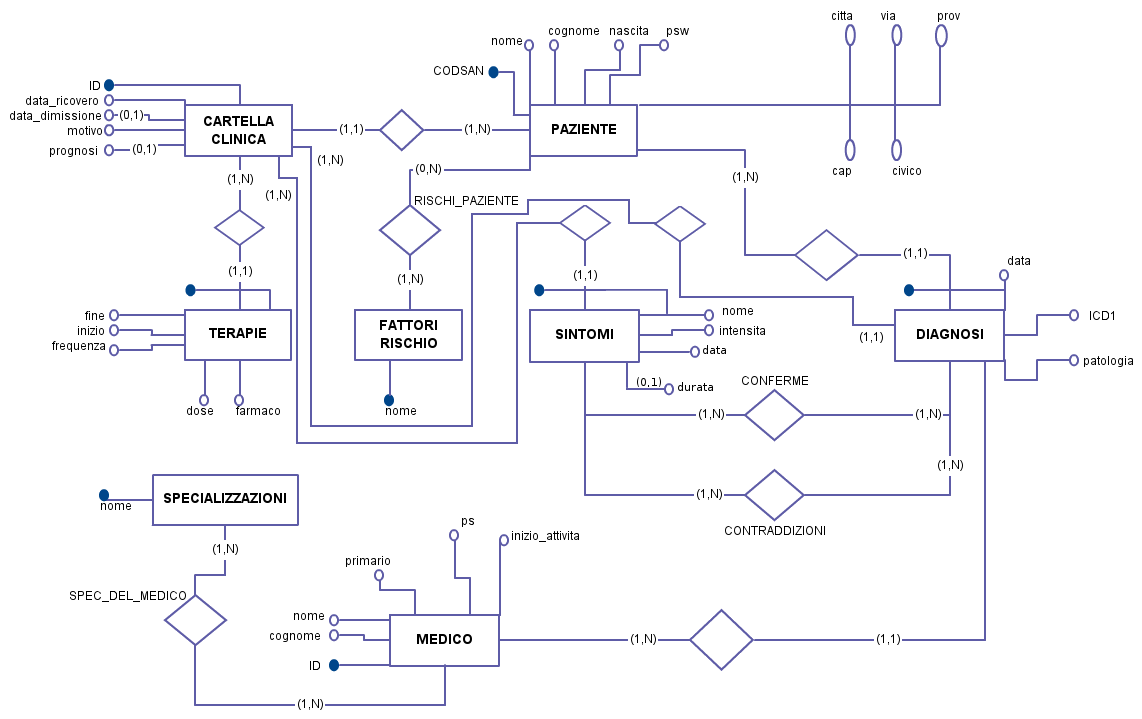
\includegraphics[scale=0.45]{ER.png}
}
    \end{center}
\vfill
\newpage
{\large Elenco delle relazioni:}\newline

\begin{enumerate}

\item Relazione TERAPIE - CARTELLA CLINICA:

\begin{itemize}[leftmargin=0.5cm, topsep=0.25cm, itemsep=0.2cm]

\item Cardinalità (1,1), una TERAPIA è associata univocamente ad una CARTELLA CLINICA
\item Cardinalità (1,N), ad una CARTELLA CLINICA può corrispondere più TERAPIE

\end{itemize}

\item Relazione CARTELLA CLINICA - PAZIENTE:

\begin{itemize}[leftmargin=0.5cm, topsep=0.25cm, itemsep=0.2cm]

\item Cardinalità (1,1), una CARTELLA CLINICA è associata univocamente ad un PAZIENTE
\item Cardinalità (1,N), ad un PAZIENTE può corrispondere più CARTELLE CLINICHE

\end{itemize}

\item Relazione CARTELLA CLINICA - SINTOMI:

\begin{itemize}[leftmargin=0.5cm, topsep=0.25cm, itemsep=0.2cm]

\item Cardinalità (1,N), ad una CARTELLA CLINICA può corrispondere uno o più SINTOMI
\item Cardinalità (1,1), un SINTOMO è associato univocamente ad una CARTELLA CLINICA

\end{itemize}

\item Relazione CARTELLA CLINICA - DIAGNOSI:

\begin{itemize}[leftmargin=0.5cm, topsep=0.25cm, itemsep=0.2cm]

\item Cardinalità (1,N), ad una CARTELLA CLINICA può corrispondere una o più DIAGNOSI
\item Cardinalità (1,1), una DIAGNOSI è associata univocamente ad una CARTELLA CLINICA

\end{itemize}

\item Relazione PAZIENTE - FATTORI RISCHIO:

\begin{itemize}[leftmargin=0.5cm, topsep=0.25cm, itemsep=0.2cm]

\item Cardinalità (0,N), ad un PAZIENTE può corrispondere nessuno o più FATTORI RISCHIO
\item Cardinalità (1,N), ad un FATTORE RISCHIO può corrispondere uno o più PAZIENTI

\end{itemize}

\item Relazione PAZIENTE - DIAGNOSI:

\begin{itemize}[leftmargin=0.5cm, topsep=0.25cm, itemsep=0.2cm]

\item Cardinalità (1,N), ad un PAZIENTE può corrispondere una o più DIAGNOSI
\item Cardinalità (1,1), una DIAGNOSI è associata univocamente ad un PAZIENTE

\end{itemize}

\item Relazione SINTOMI - DIAGNOSI:

\begin{itemize}[leftmargin=0.5cm, topsep=0.25cm, itemsep=0.2cm]

\item Cardinalità (1,N), ad un SINTOMO può corrispondere una o più DIAGNOSI
\item Cardinalità (1,N), ad una DIAGNOSI può corrispondere uno o più SINTOMI

\end{itemize}

\item Relazione DIAGNOSI - MEDICO:

\begin{itemize}[leftmargin=0.5cm, topsep=0.25cm, itemsep=0.2cm]

\item Cardinalità (1,1), una DIAGNOSI è associata univocamente ad un MEDICO
\item Cardinalità (1,N), ad un MEDICO può corrispondere una o più DIAGNOSI

\end{itemize}

\item Relazione MEDICO - SPECIALIZZAZIONI:

\begin{itemize}[leftmargin=0.5cm, topsep=0.25cm, itemsep=0.2cm]

\item Cardinalità (1,N), ad un MEDICO può corrispondere una o più SPECIALIZZAZIONI
\item Cardinalità (1,N), ad una SPECIALIZZAZIONE può corrispondere uno o più MEDICI

\end{itemize}

\end{enumerate}

\newpage

\part{Schema Logico}
    \begin{center}

    \centering
    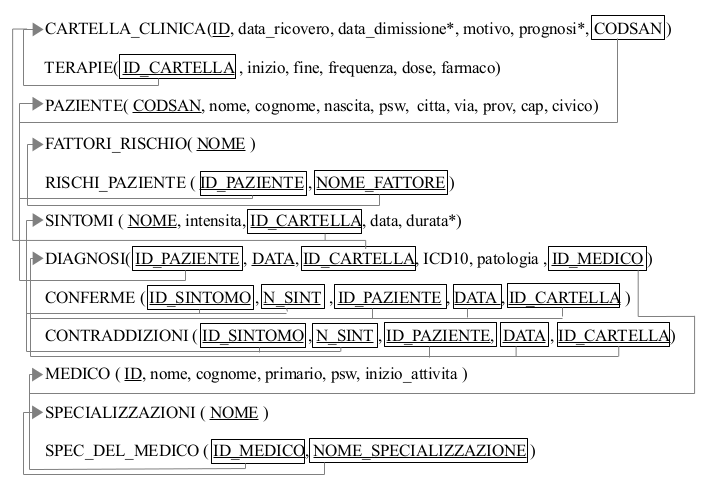
\includegraphics[scale=0.9]{schema_logico.png}

    \end{center}

Questo schema logico rappresenta una visione globale sull'elenco dei vari attributi, sulle chiavi primarie (attributi sottolineati) e sulle relazione tra di essi (i riquadri attorno al nome dell'attributo e la relativa freccia che punta alla relazione).
\newpage
\part{Page Schema}

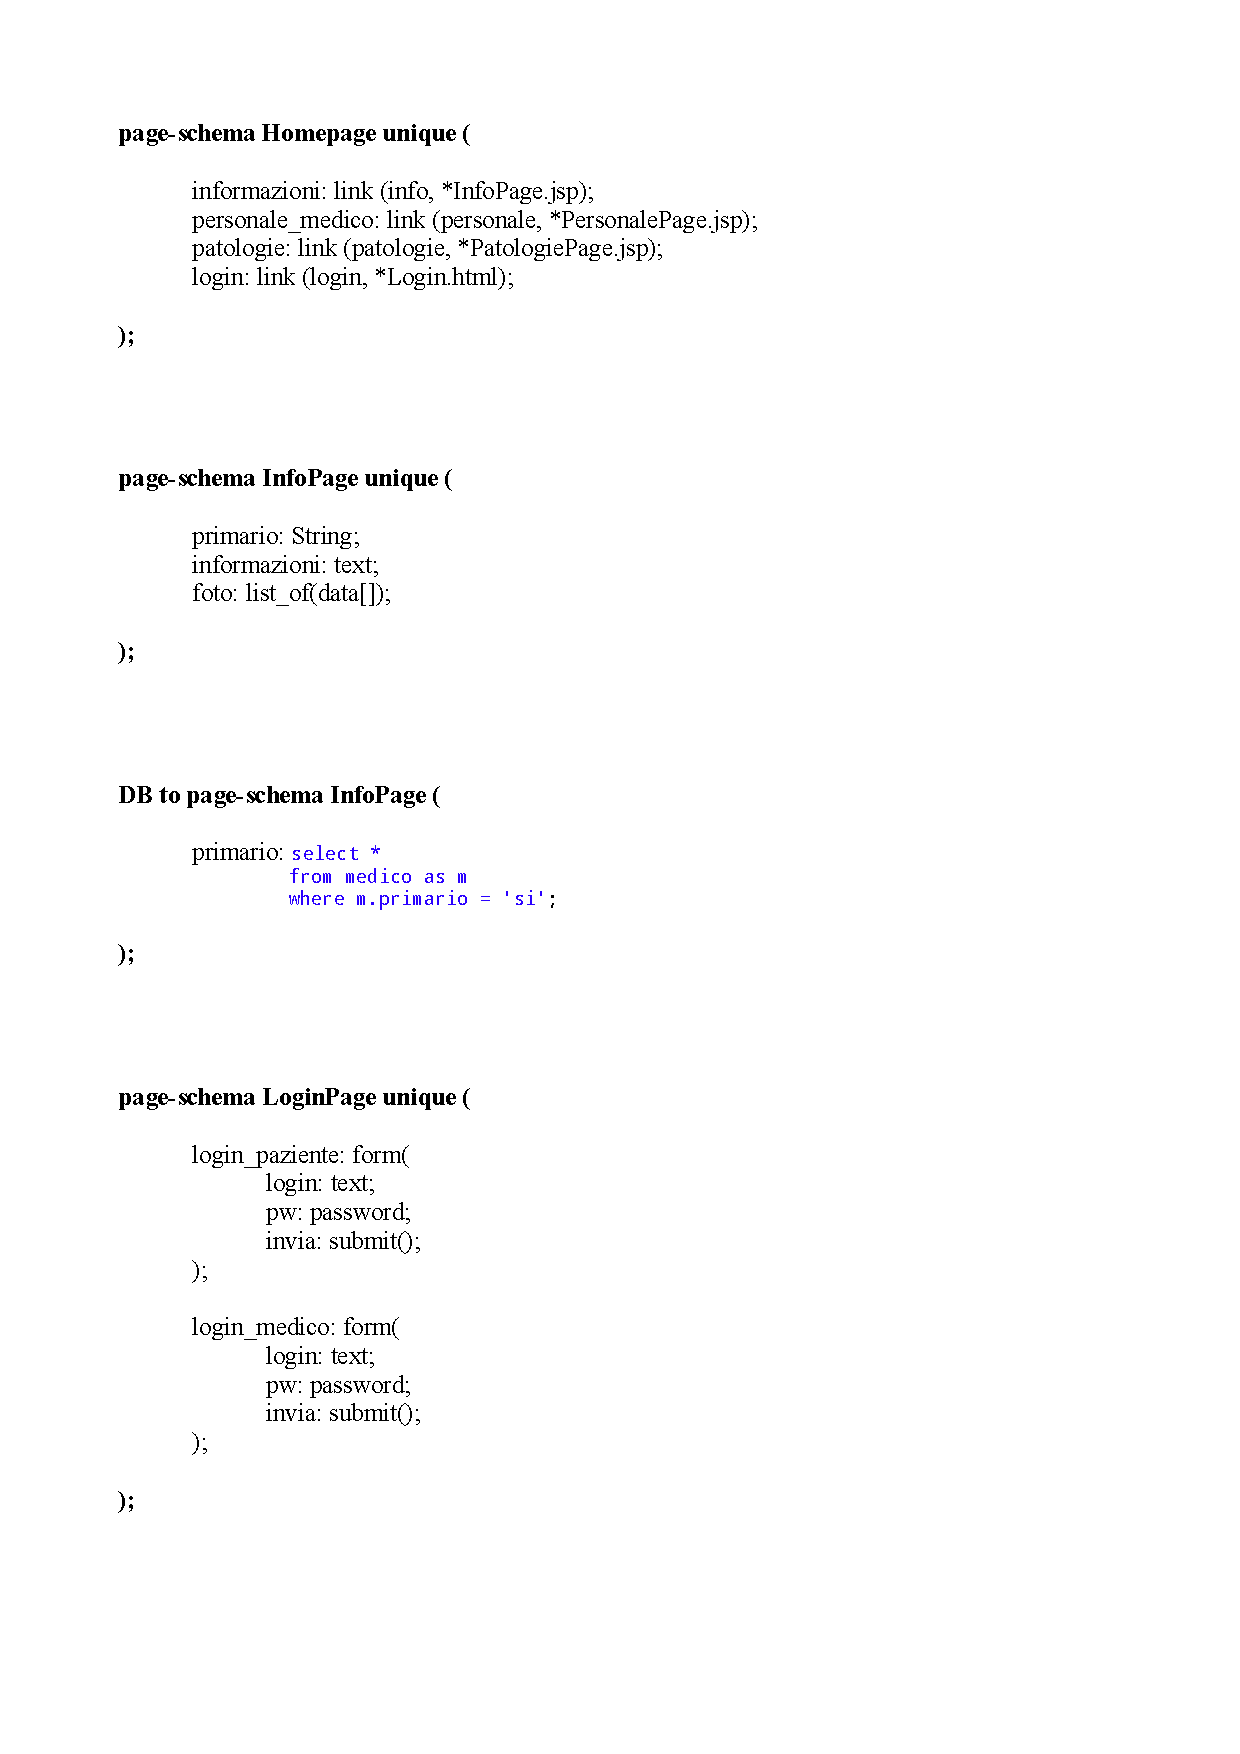
\includepdf[pages=-]{pageSchema.pdf}

\part{Strategie progettuali e considerazioni personali}

Considerazioni personali e strategie adottate durante lo sviluppo del progetto:

\begin{itemize}[leftmargin=1.5cm, topsep=0.5cm, itemsep=0.2cm]

\item Realizzazione del DB in modo tale da poter ottenere più relazioni possibili con la cartella clinica;
\item Utilizzo del metodo Hibernate durante la realizzazione del progetto in modo tale da poter semplificare le query, tenendo presente che esse restituivano tanti valori nidificati a cui ci si poteva raggiungere tramite superchiavi;
\item Durante la creazione della pagina relativa alle diagnosi (DiagnosiPage) il campo delle cartelle cliniche viene popolato tramite uno script ajax-json-jquery a seconda del paziente selezionato, in modo tale da evitare l'inserimento manuale di una cartella clinica potenzialmente errata;
\item Per la realizzazione generale della pagina web che gestisce l'intero progetto ci siamo sentiti di renderla più gradevole graficalmente inserendo uno stile di impaginazione html in formato css;
\item ECLIPSE pls!

\end{itemize}

\end{document}


